
\documentclass[
	% -- opções da classe memoir --
	article,			% indica que é um artigo acadêmico
	11pt,				% tamanho da fonte
	oneside,			% para impressão apenas no verso. Oposto a twoside
	a4paper,			% tamanho do papel. 
	% -- opções da classe abntex2 --
	%chapter=TITLE,		% títulos de capítulos convertidos em letras maiúsculas
	%section=TITLE,		% títulos de seções convertidos em letras maiúsculas
	%subsection=TITLE,	% títulos de subseções convertidos em letras maiúsculas
	%subsubsection=TITLE % títulos de subsubseções convertidos em letras maiúsculas
	% -- opções do pacote babel --
	english,			% idioma adicional para hifenização
	brazil,				% o último idioma é o principal do documento
	sumario=tradicional
	]{abntex2}

\newcommand{\matlabCodePath}{/home/clifte/git/Mestrado/Matlab/}
\newcommand{\matlabRBFCodePath}{/home/clifte/git/Mestrado/Matlab/Trabalho_RNA/trabalho2/RBF/}
% ---
% PACOTES
% ---

% ---
% Pacotes fundamentais 
% ---
\usepackage{lmodern}			% Usa a fonte Latin Modern
\usepackage[T1]{fontenc}		% Selecao de codigos de fonte.
\usepackage[utf8]{inputenc}		% Codificacao do documento (conversão automática dos acentos)
\usepackage{indentfirst}		% Indenta o primeiro parágrafo de cada seção.
\usepackage{nomencl} 			% Lista de simbolos
\usepackage{color}				% Controle das cores
\usepackage{graphicx}			% Inclusão de gráficos
\usepackage{microtype} 			% para melhorias de justificação
 
\usepackage{amsmath} 			% Equações 
\usepackage{graphicx}
\usepackage{caption}
\usepackage{subcaption}
\usepackage{tikz}
\usepackage{listings}
\usepackage[]{mcode}
\usepackage{listingsutf8}
\usepackage{epstopdf}
\usepackage{csvsimple}


% ---
		
% ---
% Pacotes adicionais, usados apenas no âmbito do Modelo Canônico do abnteX2
% ---
\usepackage{lipsum}				% para geração de dummy text
% ---
		
% ---
% Pacotes de citações
% ---
\usepackage[brazilian,hyperpageref]{backref}	 % Paginas com as citações na bibl
\usepackage[alf]{abntex2cite}	% Citações padrão ABNT


% ---

% ---
% Configurações do pacote backref
% Usado sem a opção hyperpageref de backref
\renewcommand{\backrefpagesname}{Citado na(s) página(s):~}
% Texto padrão antes do número das páginas
\renewcommand{\backref}{}
% Define os textos da citação
\renewcommand*{\backrefalt}[4]{
	\ifcase #1 %
		Nenhuma citação no texto.%
	\or
		Citado na página #2.%
	\else
		Citado #1 vezes nas páginas #2.%
	\fi}%
% ---

% ---
% Informações de dados para CAPA e FOLHA DE ROSTO
% ---
\titulo{Relatório de Trabalho 2}
\autor{David Clifte da Silva Vieira}
\local{Brasil}
\data{2014, 21 de outubro}
% ---

% ---
% Configurações de aparência do PDF final

% alterando o aspecto da cor azul
\definecolor{blue}{RGB}{41,5,195}

% informações do PDF
\makeatletter
\hypersetup{
     	%pagebackref=true,
		pdftitle={\@title}, 
		pdfauthor={\@author},
    	pdfsubject={Modelo de artigo científico com abnTeX2},
	    pdfcreator={LaTeX with abnTeX2},
		pdfkeywords={abnt}{latex}{abntex}{abntex2}{atigo científico}, 
		colorlinks=true,       		% false: boxed links; true: colored links
    	linkcolor=blue,          	% color of internal links
    	citecolor=blue,        		% color of links to bibliography
    	filecolor=magenta,      		% color of file links
		urlcolor=blue,
		bookmarksdepth=4
}
\makeatother
% --- 

% ---
% compila o indice
% ---
\makeindex
% ---

% ---
% Altera as margens padrões
% ---
\setlrmarginsandblock{3cm}{3cm}{*}
\setulmarginsandblock{3cm}{3cm}{*}
\checkandfixthelayout
% ---

% --- 
% Espaçamentos entre linhas e parágrafos 
% --- 

% O tamanho do parágrafo é dado por:
\setlength{\parindent}{1.3cm}

% Controle do espaçamento entre um parágrafo e outro:
\setlength{\parskip}{0.2cm}  % tente também \onelineskip

% Espaçamento simples
\SingleSpacing

% ----
% Início do documento
% ----
\begin{document}
% Retira espaço extra obsoleto entre as frases.


% ----------------------------------------------------------
% ELEMENTOS PRÉ-TEXTUAIS
% ----------------------------------------------------------

%---
%
% Se desejar escrever o artigo em duas colunas, descomente a linha abaixo
% e a linha com o texto ``FIM DE ARTIGO EM DUAS COLUNAS''.
% \twocolumn[    		% INICIO DE ARTIGO EM DUAS COLUNAS
%
%---
% página de titulo
\maketitle
\frenchspacing 


% ]  				% FIM DE ARTIGO EM DUAS COLUNAS
% ---

% ----------------------------------------------------------
% ELEMENTOS TEXTUAIS
% ----------------------------------------------------------
\textual

% ----------------------------------------------------------
% Introdução
% ----------------------------------------------------------
\section*{Introdução}
\addcontentsline{toc}{section}{Introdução}
Este trabalho apresenta o resultados obtidos durante o desenvolvimento da
segunda lista de exercícios propostos pelo professor Ajalmar Roccha no curso de
mestrado em Ciências da Computação do IFCE. Parte do código fonte é exibido na
forma de Apêndice ao fim do trabalho.
   Neural Networks have been extensively used in many fields due to their ability
to approximate complex nonlinear mappings directly from the input sample; and
to provide models for a large class of natural and artificial phenomena that are
difficult to handle using classical parametric techniques. There are many algorithm

\section*{RBF - Radial Basis Function}

\subsection{Teorema de Cover} As redes RBF tem como princípio a transformação
não linear das entradas para um espaço de alta dimensionalidade. Segundo o
teorema de Cover sobre a separabilidade de padrões, nesse novo espaço de alta
dimensionalidade a probabilidade de existir um hiperplano que posso separar
linearmente os dados é maior.

\begin{citacao}
Um problema complexo de classificação de padrões disposto não linearmente em um
espaço de alta dimensão tem maior probabilidade de ser linearmente separável do
que em um espaço de baixa dimensionalidade.(Cover, 1965) 
\end{citacao}

\begin{align}
P(N,m_1) = \left(\frac{1}{2}\right)^{N-1}   
\sum_{m=0}^{m_1-1}   
\binom{N-1}{m}
\label{eq:teoSepCover}
\end{align}

Na equação \ref{eq:teoSepCover}, citada no trabalho de Cover temos a
probabilidade de um padrão $x$ ser separado linearmente de $\chi=\{x_i\}_{i=1}^{N}$ após passar por uma
transformação através de uma função oculta $\phi(x)$ que mapeia o padrão $x$ em
um espaço de maior dimensionalidade.
Podemos perceber que a medida que o número de dimensões $m_1$ aumentam para uma
determinado número $N$ padrões a probabilidade resultante tende a 1.


\subsection{Mapeamento da função oculta}
Um mapeamento não linear é utilizado para realizar uma tranfomação nos dados de
classificação de forma que ele possa ser resolvido linearmente. Como visto na
sessão anterior, Cover resolveu este problema ao aumentar o número de dimensões
dos padrões.

O mapeamento é feito através do vetor $\phi(x)$.
\begin{align}
\phi(x) = [ \phi_1(x), \phi_2(x), \ldots, \phi_{m1}(x) ] 
\label{eq:phiVec}
\end{align}
Dado um vetor $x$ oriundo do espaço de entrada de dimensão $m_0$. O vetor
$\phi(x)$ realiza o mapeamento de $x$ em novo espaço de dimensão $m_1$. Como
representado na equação \ref{eq:phiVec}, $\phi(x)$ é um conjunto de funções
ocultas $\{\phi_i(x)\}^{m_1}_{i=1}$ que mapeiam o vetor $x$ no novo espaço
denominado espaço oculto ou espaço de caracaterísticas. É esperado que no espaço
de características seja possível realizar a classificação dos dados de forma
linear. O hiperplano que separa as classes é definido por
\begin{align}
\phi(x)W^t=0
\end{align} 

Desta forma temos que para $x \in \chi_1 $, $\phi(x)W^t>0$, onde $W$ é um
vetor com os termos da combinação das funções de base radial e $\chi_1$ é a
classe na qual $x$ faz parte.

\subsection{A Rede RBF}
Uma rede RBF(Radial Basis function), da mesma forma que rede MLP e ELM é
composta por três camadas.
Uma camada de entrada, camada oculta e camada de saída. A principal diferença entre
este modelo e os outros está na camada oculta que apresenta como função de
ativação uma função de base radial.

Uma função de base radial é caracterizada pelo valor aumentar ou
diminuir de acordo com a distancia ao ponto central da função. A função
gaussiana geralmente é utilizadas em redes RBFs, ela se caracteriza por valores
próximos da média apresentarem valores próximos a 1 e valores distantes da média
apresentam valores próximos a 0. Através do valor da variância é
possível controlar o raio de atuação da gaussiana como função de base
radial.

A resposta a uma entrada $x$ em uma rede RBF pode ser representada como:
\begin{align}
Y(X)=\sum^{N}_{i=1}W_i\phi(\|x-x_i\|)
\end{align}

\subsection{Treinamento da rede}
O treinamento de uma rede RBF possui duas fases. A princípio é necessário
definir os parâmetros das funções de base radial e posteriormente os pesos
utilizados nos neurônios de saída. Uma técnica geralmente utilizada para a
definição dos parâmetros das funções de base radial é o K-means, nele K
vetores médios pertecentes aos dados de treinamentos são escolhidos como centro
das funções de base radial(Bishop, 1995). Uma outra abordagem possível para a
definição dos centros das funções é realizar a subamostragem dos vetores de
entrada. Após a definição das funções de base radial resta apenas o calculo dos
pesos da camada de saída. Como dito anteriormente este problema se resume a
otimização de um classificador linear e pode ser obtido com a tecnica simples
da pseudo inversa (Haykin, 2008).
\begin{align}
W\phi=Y \\
W*\phi*\phi^{-1}=Y*\phi^{-1}\\
W=Y*\phi^{-1},\ para\ \phi\ quadrado\ ou \\
W=Y*\phi^{\dagger},\ para\ \phi\ não\ quadrado
\end{align}

\subsection{Exemplo de aplicação de uma rede RBF}
A Rede RBF será aplicada para problemas de classificação, são eles:
Problemas da iris, doenças de pele e da coluna vertebral. Para todos os
problemas a determinação dos parâmetros da rede foi feita através do algoritmo
de otimização gridSearch. Foram variados os valores de sigma e da quantidade de
neurônios afim de se obter o melhor resultado para cada problema.
Foram obtidos os seguintes resultados para os três conjuntos de dados, tabela
\ref{tab:rbfRes}.

\begin{table}[h]
\centering
\begin{tabular}{|l|l|l|l|l|l|}
\hline
DataSet          & Acurácia & nTreinamento & nTeste & nNeurônios & Sigma \\ \hline
Íris             & 0,9533   & 120          & 30     & 8          & 4,85  \\ \hline
Derme            & 0,9068   & 292          & 73     & 10         & 1,85  \\ \hline
Coluna Vertebral & 0,8226   & 248          & 62     & 12         & 4,10   \\
\hline
\end{tabular}
  
   


\caption{Resultados obtidos pelo classificador RBF.nTreinamento, nTeste e
nNeurônios são as quantidades de de dados de treinamento, quantidade de dados
de teste e quantidade de neurônios utilizados no treinamento. Sigma é o valor
de sigma utilizado na gaussiana multivariada.}
\label{tab:rbfRes}
\end{table} 
 
Foi obtido também a matriz confusão para cada conjunto de dados. Na tabela
\ref{tab:confRBFIris} temos a matriz confusão resultante do teste do treinamento
na base de dados da íris, podemos observar que há uma pequena confusão entre as
classes versicolor e virgínica. Podemos verificar nas tabelas
\ref{tab:confRBFDerme}, \ref{tab:confRBFVertebra} algo semelhante, pequenas
confusões entre as classes mais próximas.

\begin{table}[h]
\centering
\csvreader[tabular=|c|c|c|c|,
		   separator=tab,
		   late after line={\\\hline},
		   no head, table head=\hline
		   ]
{\matlabRBFCodePath saida/RBF_confusion_iris.csv} {}
{\csvcoli & \csvcolii & \csvcoliii & \csvcoliv}
\caption{Matriz confusão obtida para a base da iris}
\label{tab:confRBFIris}
\end{table} 
     
\begin{table}[h] 
\centering
\csvreader[tabular=|p{2cm}|l|p{1.8cm}|p{1.5cm}|p{1.8cm}|p{1.8cm}|p{1.8cm}|,
		   separator=tab,
		   late after line={\\\hline},
		   no head, table head=\hline
		   ] 
{\matlabRBFCodePath saida/RBF_confusion_derme.csv} {}
{\csvcoli & \csvcolii & \csvcoliii & \csvcoliv & \csvcolv & \csvcolvi &
\csvcolvii}
\caption{Matriz confusão obtida para a base de dados de doenças da derme}
\label{tab:confRBFDerme}
\end{table}



\begin{table}[h]
\centering
\csvreader[tabular=|c|c|c|c|,
		   separator=tab,
		   late after line={\\\hline},
		   no head, table head=\hline
		   ]
{\matlabRBFCodePath saida/RBF_confusion_vertebra.csv} {}
{\csvcoli & \csvcolii & \csvcoliii & \csvcoliv}
\caption{Matriz confusão obtida para a base de dados de doenças da coluna}
\label{tab:confRBFVertebra}
\end{table}


\section*{MLP - Multilayer Perceptron}

Uma rede MLP é uma rede multicamada constituída por perceptrons conectados
entre si por pesos. Os perceptrons pertencentes a rede estão conectados formando
pelo menos três camadas. A primeira é a camada de entrada, responsável por
receber os sinais de entrada, processá-lo e encaminhá-los para a camada oculta.
A segunda camada, chamada de camada oculta realiza o processamento dos dados
vindos da camada de entrada e encaminha o resultado para a camada seguinte esta
podendo ser outra camada oculta ou a camada de saída. Finalmente a camada de
saída que representa o resultado da rede. 

\begin{figure}[!htb]
	\centering
	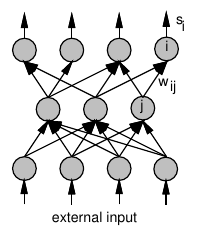
\includegraphics[width=6cm]{imagens/mlp.png}
	\caption{Rede MLP.}
	\label{fig:digraph}
\end{figure}

Na figura \ref{fig:digraph} temos uma representação de uma rede MLP.
onde $s_i$ é a camada calculada, $s_j$ é a camada anterior, $w_j$ são os pesos
da conexão e $f$ é a função de ativação do neurônio. A função de ativação
costuma ser uma sigmoíde como a tangente hiperbólica ou a logística, porém o
mais importante desta função é que ela seja diferenciável. Isso será uma
característica importante para o algoritmo Backpropagation Na equação
\ref{eq:logistica} e \ref{eq:logisticaDer} temos a função sigmóide logística e
sua derivada aplicada a um perceptron.
\begin{align}
	s_i=f(s_j*w_j)=f(net_i)=\frac{1}{1+e^{-net_i}}
\label{eq:logistica}
\end{align}

\begin{align}
	f'(s_i)=s_i*(1-s_i)
\label{eq:logisticaDer}
\end{align} 

\subsection{Backpropagation}
Durante a fase de treinamento a atualização dos pesos de forma geral é feita de
acordo com a equação \ref{eq:atualPeso}
\begin{align}
	\Delta w(t)= \eta*\frac{\delta E}{\delta w} \\
	w(t+1)=w(t)+\Delta w(t)
\label{eq:atualPeso}
\end{align}
A ideia principal do backpropagation é calcular as derivadas parcias
$\frac{\delta E}{\delta w}$ para cada peso da rede. Isso é feito através da
aplicação sucessiva da regra da cadeia.
\begin{align}
\frac{\delta E}{\delta w_{ij}}=
\frac{\delta E}{\delta s_i}
\frac{\delta s_i}{\delta w_{ij}}
\\ onde \\
\frac{\delta s_i}{\delta w_{ij}}=
\frac{\delta s_i}{\delta net_i}
\frac{\delta net_i}{\delta w_{ij}}=
f'(net_i)s_j
\end{align}

O cáculo de $\frac{\delta E}{\delta s_i}$, ou seja, a influencia da saída
$s_i$ no erro $E$ é diferente para a camada oculta e camada de saída.
Na camada de saída o cálculo de $\frac{\delta E}{\delta s_i}$ é feita da
seguinte forma.

\begin{align}
\frac{\delta E}{\delta s_i}=
\frac{1}{2}\frac{\delta (t_i-s_i)^2}{\delta s_i}=-(t_i-s_i)
\end{align}

Já para o cáculo da camada oculta deve-se reaplicar a regra da cadeia, desta
forma temos:

\begin{align}
\frac{\delta E}{\delta s_i}=
\sum_{k \in L_i} \frac{\delta E}{\delta s_k} \frac{\delta s_k}{\delta s_i}=
\sum_{k \in L_i} \frac{\delta E}{\delta s_k} \frac{\delta s_k}{\delta net_k}
\frac{\delta net_k}{\delta s_i}=
\sum_{k \in L_i} \frac{\delta E}{\delta s_k} f'(net_k)w_{ki}
\end{align}

Após o cálculo da derivadas parciais pode-se realizar a atualização dos pesos. A
atualização dos pesos é feita corrigindo seus valores somando ao gradiente
cálculado na direção oposta. Está técnica é chamada de Gradiente descendente.
\begin{align}
\Delta w(t)=-\eta * \bigtriangledown E(t)
\end{align}
\subsection{Resultados obtidos com o MLP Backpropagation}


\subsection{RProp - Resilient backpropagation}
O algoritmo RProp tem como finalidade eliminar a influência da amplitude das
derivadas parciais na atualização do peso. O RProp faz isso ao considerar que os
pesos devem ser atualizados utilizando um valor fixo, $\Delta_{ij}$ em função
apenas da direção das derivadas parciais.

\begin{align}
\Delta w_{ij}(t) = 
\begin{cases} 
		-\Delta_{ij}(t), & \mbox{se } \frac{\delta E}{\delta w_{ij}}(t)>0 \\ 
		+\Delta_{ij}(t), & \mbox{se } \frac{\delta E}{\delta w_{ij}}(t)<0 \\
		0
\end{cases}
\end{align}

Caso o valor $\Delta$ seja constante durante todo o treinamento essa regra é
chamada de Regra Manhattan.
Caso seja variável é comum seguir a seguinte regra.

\begin{align}
\Delta^{(t)}_{ij} = 
\begin{cases} 
		\eta^+*\Delta_{ij}^{(t-1)}, & \mbox{se } 
		\frac{\delta E}{\delta w_{ij}}^{(t-1)}*
		\frac{\delta E}{\delta w_{ij}}^{(t)} >0
		\\
		\eta^-*\Delta_{ij}^{(t-1)}, & \mbox{se } 
		\frac{\delta E}{\delta w_{ij}}^{(t-1)}*
		\frac{\delta E}{\delta w_{ij}}^{(t)} <0 \\
		\Delta_{ij}^{(t-1)}
\end{cases}
\end{align}
onde
$0<\eta^-<1<\eta^+$.
No inicio do treinamento todos os valores são ajustados para $\Delta_0$. Como o
valor de $\Delta$ determina o tamanho do primeiro passo de atualizaçõ este
valor deve ser escolhido de acordo com os valores iniciais dos pesos.
Para evitar que o valor dos pesos fique muito grande, é determinado um valor
máximo para $\Delta$, $\Delta_{max}$. Os valores de $\Delta_0$ e $\Delta_{max}$
geralmente são parâmetros do treinamento.
\newline
\\
    Os valores de $\Delta$ são atualizados de acordo com os valores dos
fatores $\eta^+$ e $\eta^-$. Ambos os valores são obtidos de forma empírica. Isso impôe
uma resistência a variações grandes do gradiente.Pode ser verificado
nos trabalhos de (Martin Riedmiller,1994) que o algoritmo RProp converge mais
rápido para 5 diferentes benchmarks, cada um deles. Na tabela \ref{tab:bench}
temos o quadro comparativo dos algoritmos e benchmarks. Perceba que para o
problema das 2 espirais a solução não foi obtida

\begin{table}[h]
\centering
\begin{tabular}{|l|l|l|l|l}
\cline{1-4}
               & Backpropagation   & RProp & Speedup &  \\ \cline{1-4}
10-5-10        & 121               & 19    &    6,36     &  \\ \cline{1-4}
12-2-12        & \textgreater15000 & 322   &   46,58      &  \\ \cline{1-4}
Jogo da Trilha & 98                & 23    &    4,2     &  \\ \cline{1-4}
2 Espirais     & ...               & 4987  &    -     &  \\ \cline{1-4}
\end{tabular}
\caption{Quadro comparativo de benchmarks}
\label{tab:bench}
\end{table}



\newpage

\section*{SON - Self Organize Networks} The Self-Organizing Map (SOM), commonly
also known as Kohonen network (Kohonen 1982, Kohonen 2001) is a computational
method for the visualization and analysis of high-dimensional data.
 The
objective of a Kohonen network is to map input vectors (patterns) of arbitrary
dimension N onto a discrete map The most significant difference between the
Kohonen neural network and the feed forward back propagation neural network is
that the Kohonen network trained in an unsupervised mode.
This means that the Kohonen network is presented with data, but the correct
output that corresponds to that data is not specified. Using the Kohonen network
this data can be classified into groups. We will begin our review of the Kohonen
network by examining the training process.
\subsection{Estrutura}
The Kohonen neural network works differently than the feed forward neural
network that we learned about in Chapter 5. The Kohonen neural network contains
only an input and output layer of neurons. There is no hidden layer in a Kohonen
neural network.In a Kohonen neural network only one of the output neurons
actually produces a value. Additionally, this single value is either true or
false. When the pattern is presented to the Kohonen neural network, one single
output neuron is chosen as the output neuron. Therefore, the output from the
Kohonen neural network is usually the index of the neuron (i.e. Neuron \#5) that
fired.

\section*{ELM}
   Recently, Huang et al [25], [67]proposed a new learning algorithm for Single
Layer Feedforward Neural Network architecture called Extreme Learning Ma-
chine (ELM) which overcomes the problems caused by gradient descent based
algorithms such as Back propagation applied in ANNs. ELM can significantly
reduce the amount of time needed to train a Neural Network.
  Extreme Learning Machine proposes by Huang at el [25], [29] uses Single Layer
Feedforward Neural Network (SLFN) Architecture [1]. It randomly chooses the
input weights and analytically determines the output weights of SLFN. It has much
better generalization performance with much faster learning speed.
  ELM [25], [29] designed as a SLFN with L hidden neurons can learn L distinct
samples with zero error. Even if the number of hidden neurons (L) the number
of distinct samples (N), ELM can still assign random parameters to the hidden
nodes and calculate the output weights using pseudoinverse of H giving only a
small error $\in > 0 $.

   Theorem 1: (Liang et.al.[49]) Let an SLFN with Ä additive or RBF hidden
nodes and an activation function ´Üµ which is infinitely differentiable in any
interval of R be given. Then, for arbitrary Ä distinct input vectors Ü Ü ¾
ÊÒ        ½ ¡¡¡ Ä      and ´       µ Ä ½ randomly generated with any continuous
probability distribution, respectively, the hidden layer output matrix is invertible
with probability one, the hidden layer output matrix H of the SLFN is invertible

   Theorem 2: (Liang et.al.[49])Given any small positive value               ¼ and
activation function ´Üµ        Ê      Ê which is infinitely differentiable in any
interval, there exists Ä      Æ such that for Æ arbitrary distinct input vectors
 Ü Ü ¾ ÊÒ         ½ ¡ ¡ ¡ Ä , for any ´      µ Ä ½ randomly generated according to
any continuous probability distribution    with probability
one.
   Since the hidden node paremeters of ELM need not be tuned during training
and since they are simply assigned with random values, eqn (5) becomes a linear
system and the output weights can be estimated as follows.

% --- 
% Finaliza a parte no bookmark do PDF, para que se inicie o bookmark na raiz
% ---
\bookmarksetup{startatroot}% 
% ---


\begin{citacao}

\end{citacao}


% ]  				% FIM DE ARTIGO EM DUAS COLUNAS
% ---

% ----------------------------------------------------------
% Referências bibliográficas
% ----------------------------------------------------------
\bibliography{pdi}
Bishop, C.M., 1995, "Neural Networks for Pattern Recognition" (first ed.),
Oxford University Press Inc., New York, USA, 482 p.
 @MISC{Riedmiller94advancedsupervised,
    author = {Martin Riedmiller},
    title = {Advanced Supervised Learning in Multi-layer Perceptrons - From Backpropagation to Adaptive Learning Algorithms},
    year = {1994}
}
%"http://galaxy.agh.edu.pl/~vlsi/AI/backp_t_en/backprop.html"
%http://jeremykun.com/2012/12/09/neural-networks-and-backpropagation/

 
% ----------------------------------------------------------
% Glossário
% ----------------------------------------------------------
%
% Há diversas soluções prontas para glossário em LaTeX. 
% Consulte o manual do abnTeX2 para obter sugestões.
%
%\glossary

% ----------------------------------------------------------
% Apêndices
% ----------------------------------------------------------

% ---
% Inicia os apêndices 
% ---
\begin{apendicesenv} 

% ----------------------------------------------------------
\chapter{Código fonte: Translação, Rotação e Redimensionamento}
\label{apend:transRotRed}

	
 	\lstset{extendedchars=true,inputencoding=utf8/latin1}
 	\lstinputlisting[frame=single,
 					 numbers=left]{\matlabCodePath
 	Trabalho_PDI/q11/topico11.m}



\end{apendicesenv}
% ---

% ----------------------------------------------------------
% Anexos
% ----------------------------------------------------------
\cftinserthook{toc}{AAA}


% ---
% Inicia os anexos
% ---
%\anexos
%\begin{anexosenv}
%\chapter{}
%\end{anexosenv}

\end{document}
